\subsection{Simulation of MS-BLDC}

Figure \ref{fig:msbldc-model} shows a model of the MS-BLDC in ADS.

\begin{figure}[h t b p]
	\centering
	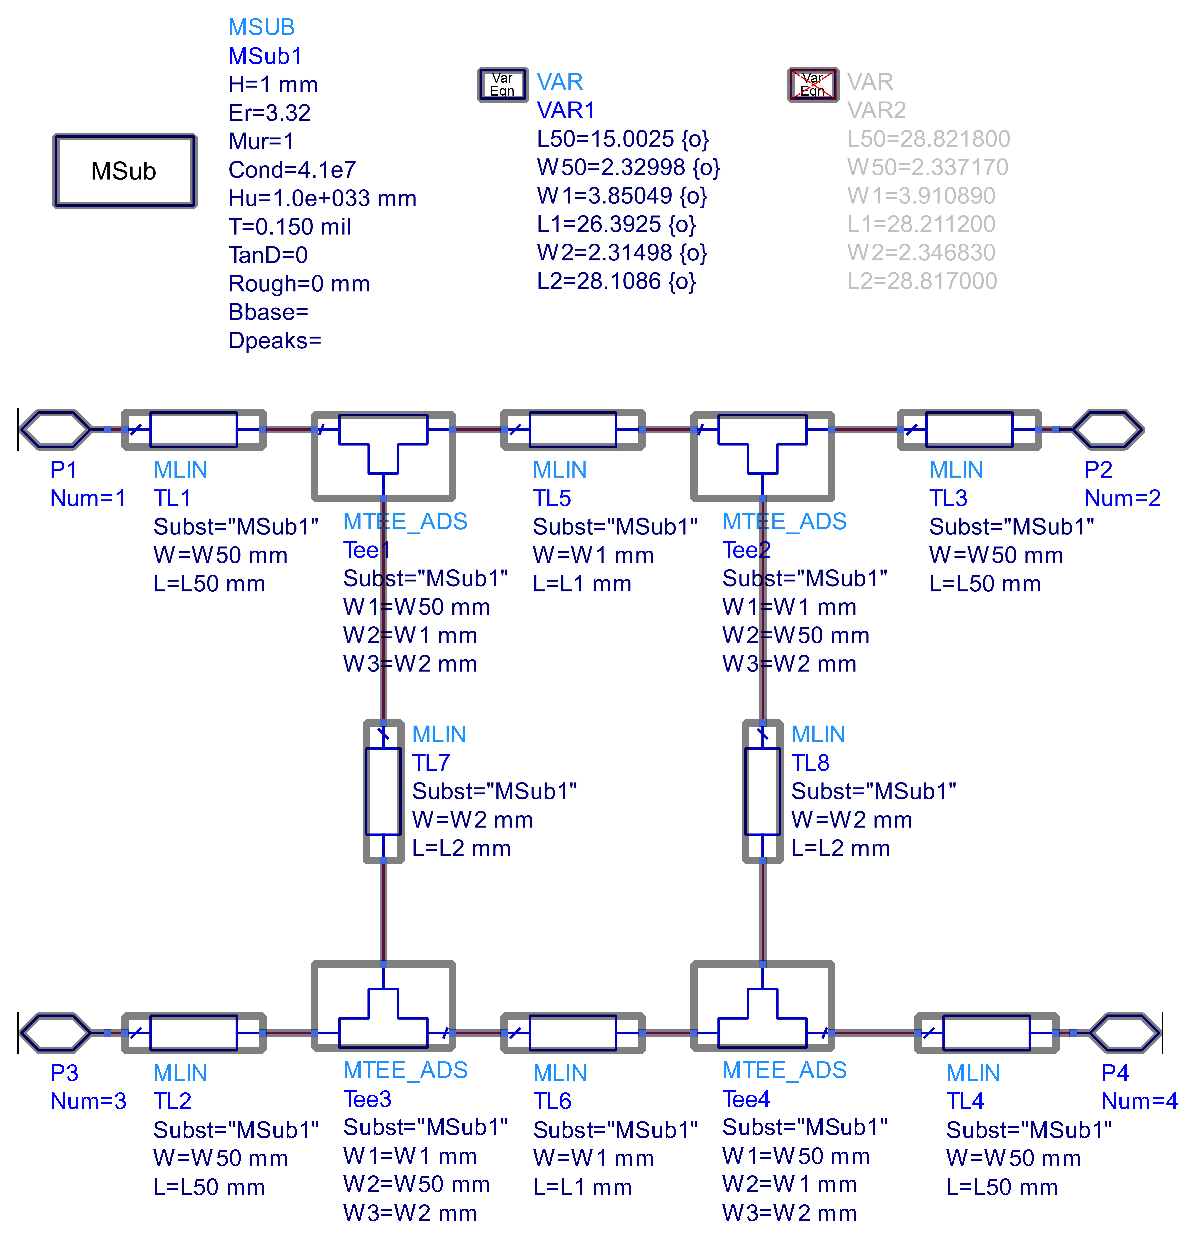
\includegraphics[width=\textwidth,keepaspectratio]{figures/msbldc-model.eps}
	\caption{Model of Microstrip branch-line directional coupler in ADS.}
	\label{fig:msbldc-model}
\end{figure}

Figure \ref{fig:41_21_3dB} shows a simulation of S(2,1) and S(4,1) in ADS.
The markers indicate the peak values.
We see that the components are in fact not exactly \SI{-3}{\decibel} at \SI{1.6}{\giga\hertz}.
As can be seen from figure \ref{fig:41_21_phase}, the two components are approximately \SI{90}{\degree} out of phase.

\begin{figure}[h t b p]
	\centering
	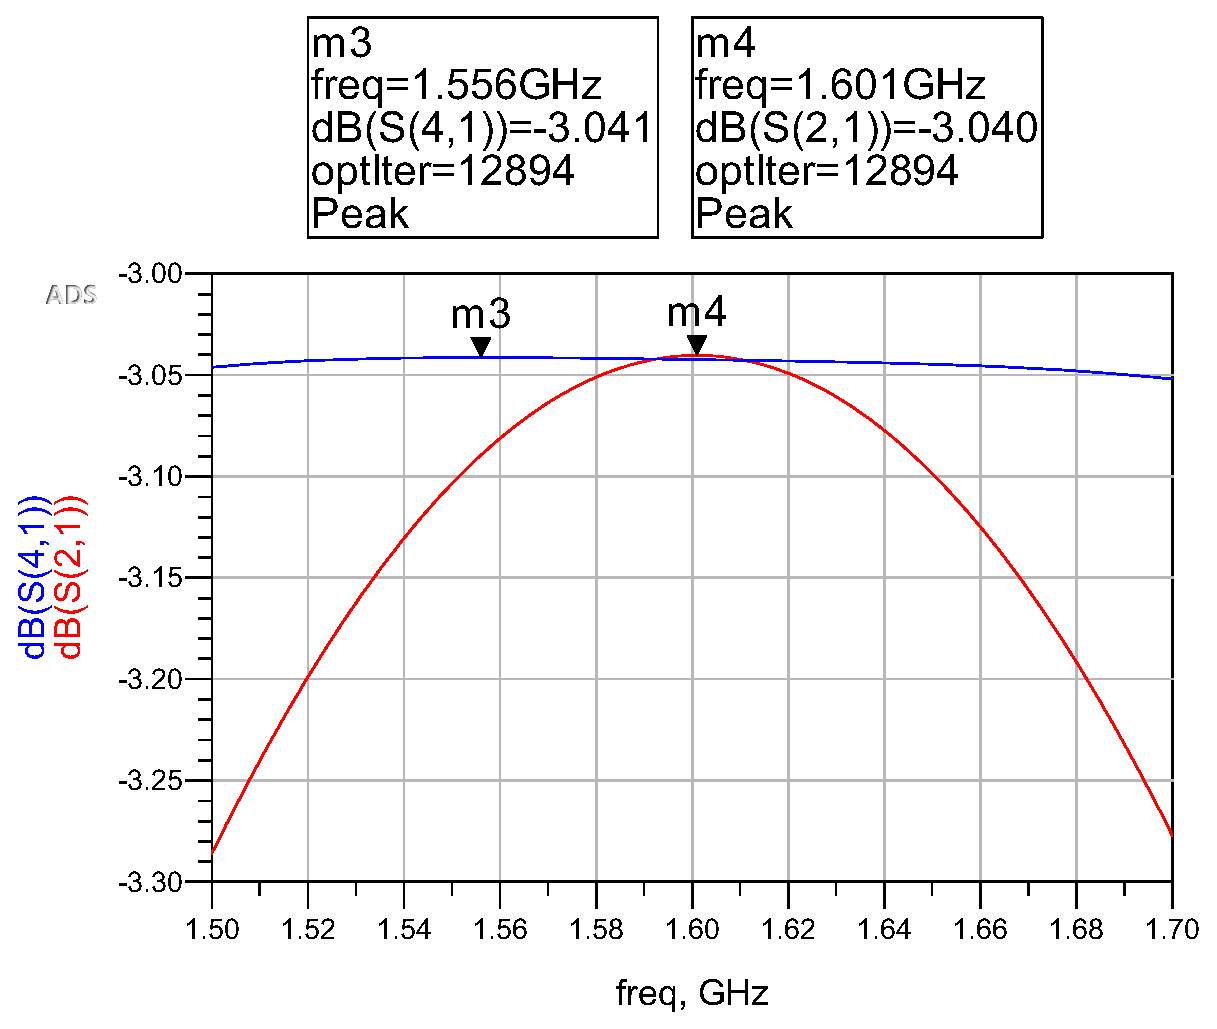
\includegraphics[width=0.8\textwidth,keepaspectratio]{figures/41_21_3dB.eps}
	\caption{Simulated S-matrix components S(2,1) and S(4,1).}
	\label{fig:41_21_3dB}
%\end{figure}
%
%\begin{figure}[h t b p]
%	\centering
	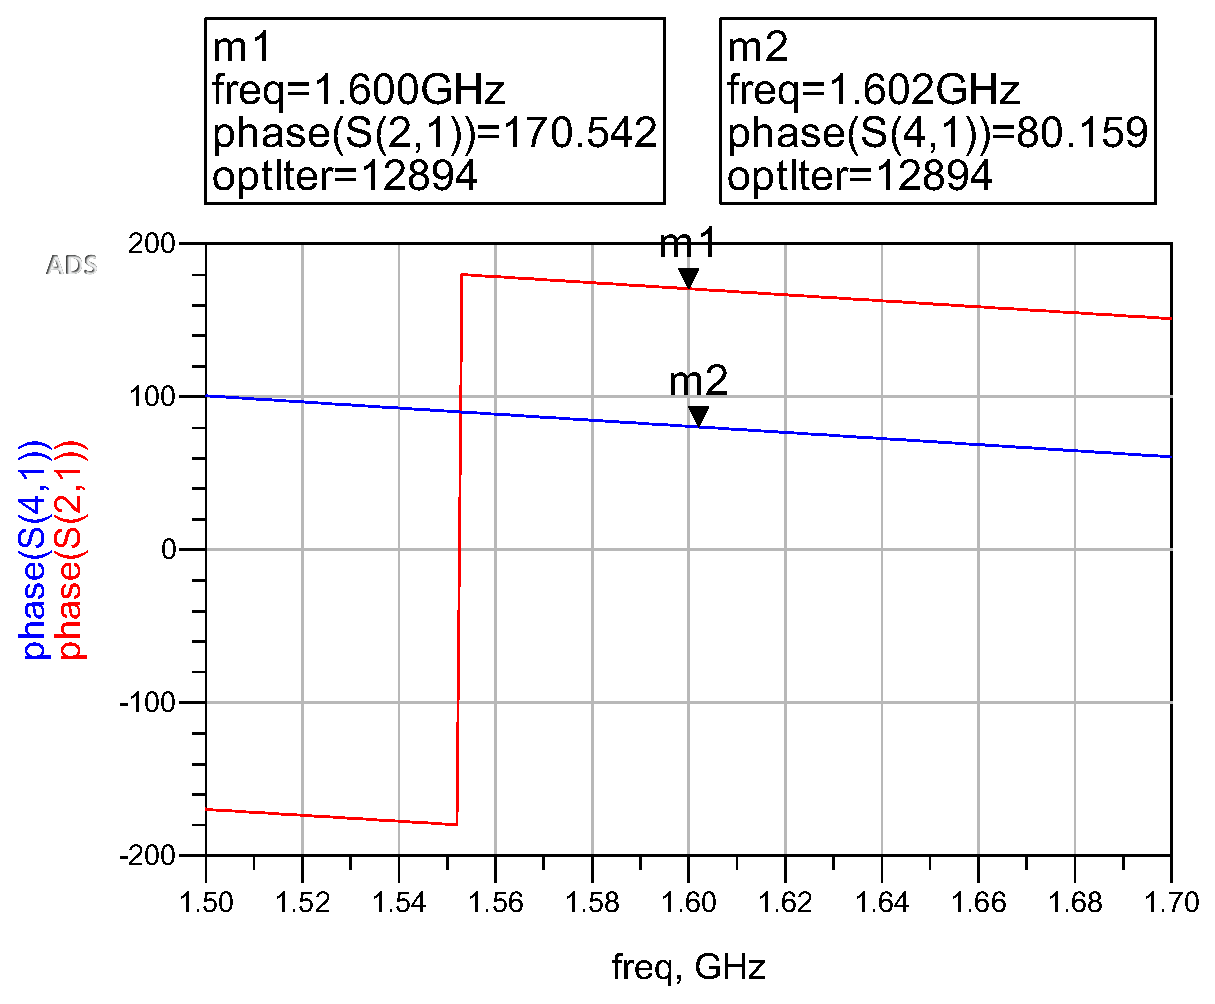
\includegraphics[width=0.8\textwidth,keepaspectratio]{figures/41_21_phase.eps}
	\caption{Simulated S(2,1) and S(4,1) phase difference.}
	\label{fig:41_21_phase}
\end{figure}